% Implementation
% Remember code snippets
% Services
% Authentication
% Transactions
% Testing
%%% what testing framework(s) did we use and why?
%%% Reasoning over these 
%%% Choice and reason for choice
%%% Results from testing
% Exception handling
% Performance
\chapter{Implementation}\label{ch:implementation}
I dette kapitel vil der blive beskrevet hvordan arkitekturen og features er implementeret. Dette vil omfatte Database, DAO, Services, Web, tests, og det landkort der er brugt til at afkryde lokationer.

\section{Database og persistence}\label{sec:database}

\subsection{SQL og DAO}\label{sec:sqlOgDao}
Eftersom der i dette projekt bruges ADO.NET direkte, uden nogen ORM eller lignende, betyder det at vi skal skrive vores egne SQL og DAO metoder. Måden dette er implementeret på er ved brug af DAO interfaces og statiske properties, som hver returnerer den tilsvarende interface. Disse interfaces, der beskriver metoderne som forventer en specifik DAO metode, og ligesom andre C\# interfaces er dette uafhængigt af den implementerede logik.
Denne metode har 2 primære fordele. Den ene fordel er, at vi nemt kan oprette mocking-klasser af vores DAO-klasser. Mocking-klasserne vil accepteres som DAO-klasser i et unit testing miljø. Et eksempel på dette kan ses i \texttt{ImageControllerSpec} \ref{lst:imageControllerSpec}.
Den anden fordel er lav kobling mellem logikken i vores DAO metoder og resten af koden. Dette kan være en kæmpe fordel, såfremt den nuværende implementation af Microsoft SQL på et tidspunkt skal udskiftes med en anden implementation. Skulle man implementere f.eks. MySQL\cite{mysql} fx ville det ikke være svært at implementere dette, eftersom al kode, der kalder DAO metoder, kalder dem gennem interfaces. Dette vil sige at alle ændringer i koden kun vil ske i QWest.DataAccess. Et eksempel på en DAO interface med tilsvarende egenskab kan findes i \texttt{QWest.DataAccess.DAO.IProgressMap} \ref{lst:progressMapDaoInterface}.
Dette projekt gør brug af en Microsoft SQL database, så derfor er egenskaben som standard sat til MsSQL implementationen af interfacen.

\begin{listing}[p]
    \begin{minted}
    [
        frame=lines,
        framesep=2mm,
        baselinestretch=1.2,
        bgcolor=LightGray,
        fontsize=\footnotesize,
        linenos,
        breaklines
    ]{csharp}
namespace QWest.Api.Tests {
    [TestFixture]
    public class ImageControllerSpec {
        public class ImageRepoMock : DAO.IImage {
            public Dictionary<int, byte[]> ImageDictionary { get; set; }
            public Task<byte[]> Get(int id) {
                return Task.FromResult(ImageDictionary[id]);
            }
        }
        [Test]
        public async Task NullReturnsValidImage() {
            ImageController imageController = new ImageController();
            imageController.ImageRepo = new ImageRepoMock();
            byte[] bytes = await (await imageController.Get(null)).Content.ReadAsByteArrayAsync();
            Assert.IsNotEmpty(bytes);
        }
        [Test]
        public async Task ReturnsCorrectImage() {
            byte[] expected = new byte[] { 1, 2, 3 };
            ImageController imageController = new ImageController();
            imageController.ImageRepo = new ImageRepoMock {
                ImageDictionary = new Dictionary<int, byte[]> {
                    {5, expected }
                }
            };
            byte[] bytes = await (await imageController.Get(5)).Content.ReadAsByteArrayAsync();
            Assert.AreEqual(expected, bytes);
        }
    }
}
\end{minted}
    \caption{QWest.Api.Tests.ImageControllerSpec\label{lst:imageControllerSpec}}
\end{listing}

\begin{listing}[p]
    \begin{minted}
    [
        frame=lines,
        framesep=2mm,
        baselinestretch=1.2,
        bgcolor=LightGray,
        fontsize=\footnotesize,
        linenos,
        breaklines
    ]{csharp}
namespace QWest.DataAccess {
    public static partial class DAO {
        public interface IProgressMap {
            Task<ProgressMap> Get(User user);
            Task<ProgressMap> Get(ProgressMap map);
            Task<ProgressMap> Get(int id);
            Task<ProgressMap> GetByUserId(int userId);
            Task Update(int id, List<int> additions, List<int> subtractions);
            Task Update(ProgressMap map);
        }
        public static IProgressMap ProgressMap { get; set; } = new Mssql.ProgressMapImpl(ConnectionWrapper.Instance);
    }
}
\end{minted}
    \caption{ProgressMap DAO interface\label{lst:progressMapDaoInterface}}
\end{listing}

\subsubsection{DbRep pattern}\label{sec:dbRep}
DbRep, en forkortelse for Database Representation, og er et designmønster vi har "opfundet". Den bruges i mange af projektets DAO metoder, fordi DbRep er et god designmønster til at stoppe kodeduplikation når det kommer til \texttt{select} DAO metoder.
Alt i alt består dette designmønster af at lave en klasse, som reflekterer resultatet af en SQL Select-metode. DbRep klassens constructor tager imod en individuel row, som i C\# vil være i form af en \texttt{SqlDataReader}. Denne udpakker hver row til en property in denne klasse. Klassen skal så repræsentere Select resultatet og constructoren skal udpakke resultatet til properties i denne klasse.
Indtil videre hjælper denne klasse med ikke at duplikere koden for udpakningen af SQL resultater, men der kan også kaldes en metode på klassen, ofte kaldet \texttt{ToModel} som returnerer den model klasse some vores DAO interface kræver at vi returnerer.
Dette designmønster kan gøre DAO metode-skrivning nemmere, eftersom udpakningen og konstruktionen af den model klassen der skal returneres allerede eksistere og vær DAO metode kan fokuseser på SQL'en.
En anden god fordel er at den splitter udpakning af data og mutering af data i to forskellige metoder. Dette er vigtigt eftersom vi gerne vil bruge så lidt tid som muligt med SQL forbindelsen åben og det er kun udpakningen af data der kræver dette.
Et eksempel på en DbRep er PostDbRep \ref{lst:postDbRep}. Constructoren's job er at udpakke værdierne og intet andet, eftersom der er en SQL forbindelse åben. Data mutationen sker i ToModel(), hvor vi først skal finde ud af om en Post var lavet af en User eller en Group. Der er komma seperarede strenge og JSON der skal parses, hvilket ikke burde gøres mens der er en utrolig dyr SQL forbindelse åben.

\begin{listing}[p]
    \begin{minted}
    [
        frame=lines,
        framesep=2mm,
        baselinestretch=1.2,
        bgcolor=LightGray,
        fontsize=\footnotesize,
        linenos,
        breaklines
    ]{csharp}
[Serializable]
internal class PostDbRep : IDbRep<Post> {
    //deleted properties for readability in this snippet
    public PostDbRep(SqlDataReader reader) {
        int i = 0;
        Id = reader.GetSqlInt32(i++).Value;
        Content = reader.GetSqlString(i++).Value;
        UserId = reader.GetSqlInt32(i++).NullableValue();
        GroupId = reader.GetSqlInt32(i++).NullableValue();
        PostTime = reader.GetSqlInt32(i++).Value;
        Location = reader.GetSqlString(i++).NullableValue();
        Username = reader.GetSqlString(i++).NullableValue();
        PasswordHash = reader.GetSqlBinary(i++).NullableValue();
        Email = reader.GetSqlString(i++).NullableValue();
        UserDescription = reader.GetSqlString(i++).NullableValue();
        SessionCookie = reader.GetSqlBinary(i++).NullableValue();
        ProfilePicture = reader.GetSqlInt32(i++).NullableValue();
        Name = reader.GetSqlString(i++).NullableValue();
        CreationTime = reader.GetSqlInt32(i++).NullableValue();
        GroupDescription = reader.GetSqlString(i++).NullableValue();
        Images = reader.GetSqlString(i++).NullableValue();
        Members = reader.GetSqlString(i++).NullableValue();
    }

    public Post ToModel() {
        User userAuthor = null;
        Group groupAuthor = null;
        if (UserId != null) {
            userAuthor = new User(Username, PasswordHash, Email, UserDescription, SessionCookie, UserId) {
                ProfilePicture = ProfilePicture
            };
        }
        else if (GroupId != null) {
            groupAuthor = new Group(Name, (int)CreationTime, GroupDescription, null, Members.MapValue(UserDbRep.FromJson).Select(x => x.ToModel()), GroupId);
        }
        else {
            throw new ArgumentException("in this post the author is neither a user or group");
        }
        return new Post(Content, userAuthor, groupAuthor, PostTime, Images.MapValue(x => x.Split(',').Select(y => int.Parse(y)).ToList()), Location.MapValue(x => GeopoliticalLocationDbRep.ToTreeStructureFirst(GeopoliticalLocationDbRep.FromJson(x))), Id);
    }
}
\end{minted}
    \caption{PostDbRep\label{lst:postDbRep}}
\end{listing}

\subsection{Migration og backups}\label{sec:migration}
QWest bruger et Database Migration Pattern\cite{datamigration} til at håndtere database ændringer.
Database Migration betyder, at i stedet for at have et færdiggjort og definitivt SQL script til at sætte databasen op, så er der mange SQL scripts, som eksekveres i specifik rækkefølge. Dette har en massiv fordel i forhold til ét kompliceret, færdiggjort og definitivt SQL script, da der kan tilføjes ændringer til databasens tabeller uden at slette al data i databasen.

Dette er utrolig vigtigt for den agile udviklings metode, hvilket kræver et development-feedback loop mellem udviklere og brugere. For at dette kan være en realitet, kræver det at applikationen har persistens mellem opdateringer for ikke at geive en forfærdelig brugeroplevelse.

For at undgå at eksekvere en migration som allerede er i databasen, er der oprettet en ekstra tabel kaldet \texttt{info} med rækken \texttt{schema\_version}. Denne holder styr på hvad nummeret var på den seneste migration der blev eksekveret. Dette tal kan så bruges til at versionstjekke, også kaldet Row-versioning\cite{rowversioning}.

QWest's migrationer kan alle sammen findes i QWest.DataAcess/Migrations, og er navngivet efter rækkefølgen de skal eksekveres i. Det starter ved \texttt{1.sql} og ender på nuværende tidspunkt ved \texttt{20.sql}

Efter migrationsprocessen i QWest, indsættes også backup af geopolitisk data,hvis intet geopolitisk data kan findes i databasen. Dette skyldes tildels testing årsager, eftersom vores integration-tests kan finde på at slette alle tabeller i databasen, hvilket ville slette denne næsten statiske data. 

\section{Services}\label{sec:servicesImp}
QWest er en applikation bestående af services, enten skrevet i node.js\cite{nodejs} eller C\#. Som nævnt i \ref{sec:servicesArc} er disse services henholdsvis \texttt{QWest.Api}, \texttt{QWest.Web}, \texttt{QWest.Email}.
Ved start af QWest kaldes disse services fra \texttt{QWest.Services.Run}, hvor \texttt{WebSerivce} og \texttt{EmailSerivce} kaldes som NodeJS services, og \texttt{ApiService} og \texttt{AdminService} kaldes som C\# services. 
Som nævnt i \ref{sec:servicesArc} er \texttt{QWest.Api} den service som forbinder front-end med resten af systemet og databasen. Hvis der eksempelvis er oprettet et opslag på front-end af brugeren, skal opslaget sendes til systemet som så kan lagre det i databasen, så det senere kan vises når brugeren efterspørger det. Implementationen af dette vil blive gennemgået i næsten afsnit \ref{sec:backend}.

\section{Web design}\label{sec:webdesign}
\subsection{Front-end and usability}\label{sec:frontend}
Som nævnt tidligere vil der blive taget udgangspunkt i eksemplet med oprettelse af et opslag. Dette opslag kan oprettes i browseren på brugerens profil, som det ses på figur \ref{fig:frontend}.

\begin{figure}
    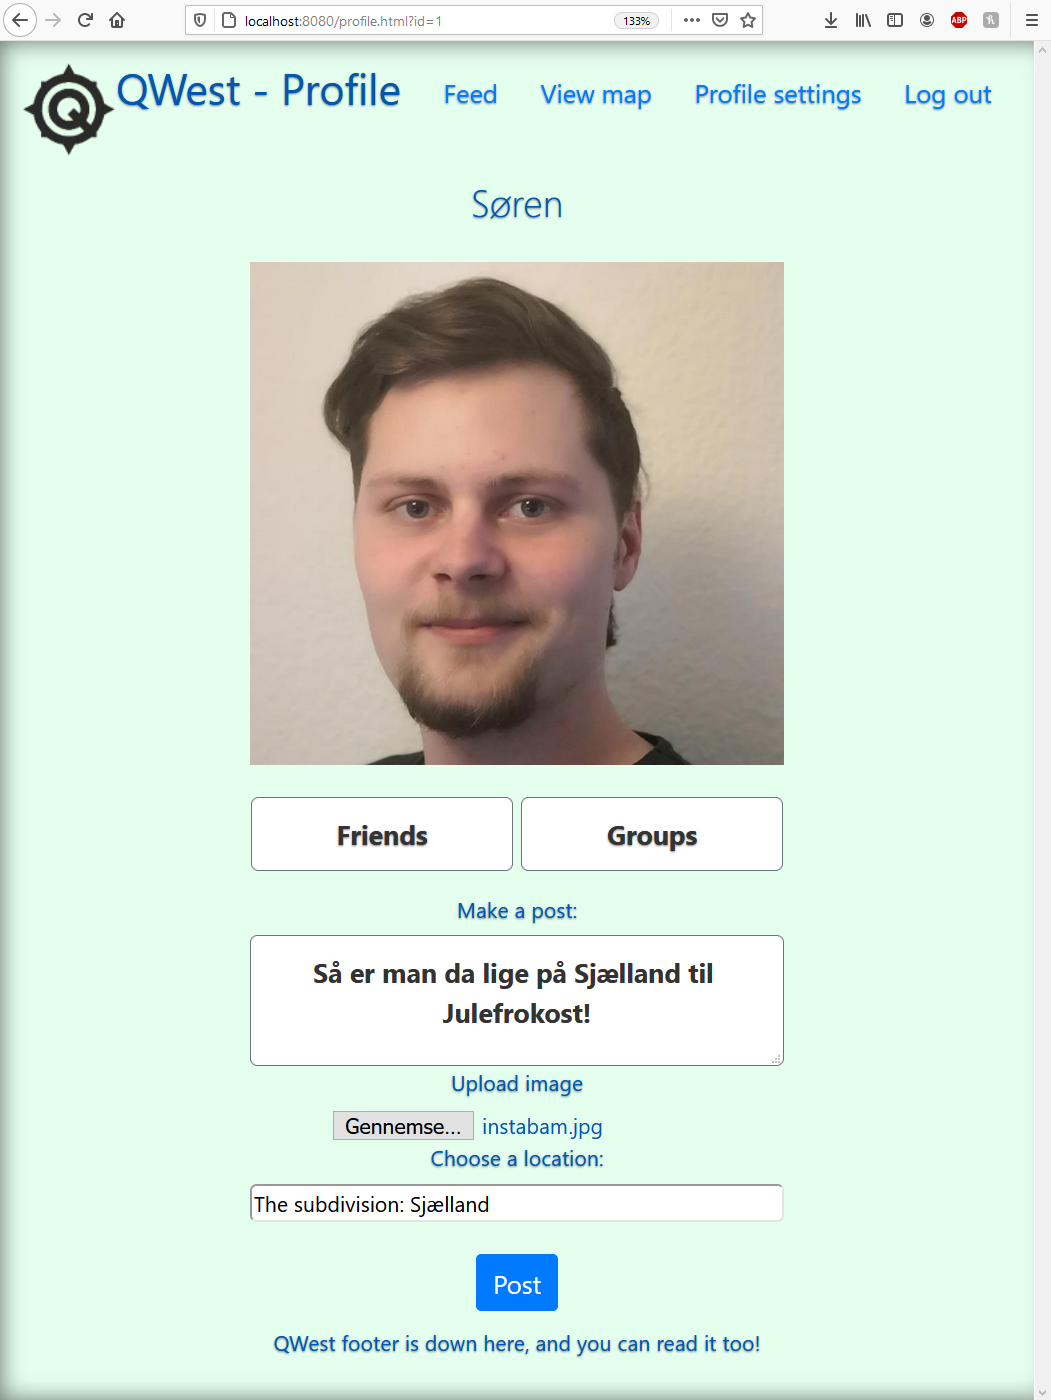
\includegraphics[width=\linewidth]{front-end.png}
    \caption{QWest - Profile, hvor brugeren kan oprette et opslag.}
    \label{fig:frontend}
\end{figure}

Alt er centreret på forsiden og både tekst og knapper er gjort store for at øge brugervenligheden. Det er muligt at tilføje beskrivelse, billede og lokation på hvert opslag, og når man trykker på "Post" knappen, skal opslaget så håndteres af back-end. 

\subsection{Back-end and logic}\label{sec:backend}

\begin{listing}[p]
    \begin{minted}
    [
        frame=lines,
        framesep=2mm,
        baselinestretch=1.2,
        bgcolor=LightGray,
        fontsize=\footnotesize,
        linenos,
        breaklines
    ]{html}
<div id="post-container">
    <label>Make a post:</label>
    <br/>
    <textarea id="post-contents" text="" placeholder="Write your post here..." class="btn btn-lg btn-secondary"></textarea>            
    <br/>
    <div class="w3-container" id="upload-file">
        <label for="file" id="image-label">Upload image</label>
        <input type="file" id="post-images" />
    </div>
    <label>Choose a location:</label>
    <div id="geopolitical-location-autocomplete"></div>
    <br>
    <button class="btn btn-primary" id="post-button">Post</button>
</div>
\end{minted}
\caption{post-container i HTML front-end.\label{lst:post-container}}
\end{listing}

I \ref{lst:post-container} er de relevante inputs textarea post-contents som er beskrivelsen af opslaget, input post-images som indeholder billedet, og geopolitical-location-autocomplete som indeholder lokationen. 
Disse inputs læses så af Javascript, som opretter et promise med beskrivelse, billede og lokation.

\begin{listing}[p]
    \begin{minted}
    [
        frame=lines,
        framesep=2mm,
        baselinestretch=1.2,
        bgcolor=LightGray,
        fontsize=\footnotesize,
        linenos,
        breaklines
    ]{javascript}
    postButton.on("click", async () => {
        const request = await POST.Post.Upload({
            contents: postContents.val(),
            location: selectedGeopoliticalLocation ? selectedGeopoliticalLocation.id : null,
            images: await Promise.all(Array.from(postImages[0].files).map(blobToBase64))
        })
        if (request.status === 200) {
            window.location.reload();
            return;
        }
        console.log(request.status)
        console.log(response.data)
    })
\end{minted}
\caption{Javascript logik til oprettelse af opslag.\label{lst:javascript-post}}
\end{listing}

Som det kan ses på linje 2 kaldes Post.Upload() metoden fra QWest.Api, hvor der sendes contents, location og images. Herefter checkes for om forespørgslen gik igennem korrekt - hvis ikke sendes fejl til log. 

\begin{listing}[p]
    \begin{minted}
    [
        frame=lines,
        framesep=2mm,
        baselinestretch=1.2,
        bgcolor=LightGray,
        fontsize=\footnotesize,
        linenos,
        breaklines
    ]{csharp}
[HttpPost]
[ResponseType(typeof(Post))]
public async Task<HttpResponseMessage> Upload([FromBody] UploadArgument upload) {
    User user = Request.GetOwinContext().Get<User>("user");
    if (user == null) {
        return new HttpResponseMessage(HttpStatusCode.Unauthorized);
    }
    List<byte[]> images = await upload.ParseImages();
    string contents = upload.contents.Trim();
    Post post;
    if (upload.groupAuthor == null) {
        post = await PostRepo.Add(contents, user, images, upload.location);
    }
    else {
        int groupAuthor = (int)upload.groupAuthor;
        if (await GroupRepo.IsMember(groupAuthor, user)) {
            post = await PostRepo.AddGroupAuthor(contents, groupAuthor, images, upload.location);
        }
        else {
            return new HttpResponseMessage(HttpStatusCode.Unauthorized);
        }
    }
    return Request.CreateResponse(HttpStatusCode.OK, post);
}
\end{minted}
\caption{Post.Upload metoden, som forefindes i QWest.Api.PostController.\label{lst:post-controller}}
\end{listing}

På kodestykket \ref{lst:post-controller} ses Post.Upload metoden nævnt tidligere. Denne er ansvarlig for at modtage et UploadArgument, som indeholder opslagets informationer, henholdsvis billeder, beskrivelse, lokation og forfatter (bruger eller gruppe). På linje 13 og 18 kaldes PostRepo.Add. PostRepo er en intern klasse, som er DAO interfacet. Interfacet \texttt{IPost} under DAOPost indeholder altså de forskellige metoder såsom Add, Get, Update og andre. Som nævnt tidligere bruger selve implementationen af interfacet Microsoft SQL, og implementationen forefindes under \texttt{PostImpl} som findes under QWest.DataAccess. 

\begin{listing}[p]
    \begin{minted}
    [
        frame=lines,
        framesep=2mm,
        baselinestretch=1.2,
        bgcolor=LightGray,
        fontsize=\footnotesize,
        linenos,
        breaklines
    ]{csharp}
public Task<Post> Add(string contents, User user, List<byte[]> images, int? locationId) {
    return AddUserAuthor(contents, (int)user.Id, images, locationId);
}

public async Task<Post> AddUserAuthor(string contents, int userId, List<byte[]> images, int? locationId) {
    string query = $@"
DECLARE @post_id INT;
INSERT INTO posts
(content, users_id, post_time, location)
VALUES
(@content, @user_id, @post_time, @location);
SET @post_id = CAST(scope_identity() AS INT);
" +
    string.Join("", images.Select((_, i) => $@"
INSERT INTO images
(image_blob)
VALUES
(@image_blob{i});

INSERT INTO posts_images
(posts_id, images_id)
VALUES
(@post_id, (SELECT CAST(scope_identity() as int)));
")) +
    $@"
SELECT
{PostDbRep.SELECT_ORDER}
FROM posts
LEFT JOIN users
ON
users.id = posts.users_id
LEFT JOIN groups
ON
groups.id = posts.groups_id
WHERE posts.id = @post_id
";
    return (await _conn.Use(query, async stmt => {
        stmt.Parameters.AddWithValue("@content", contents);
        stmt.Parameters.AddWithValue("@user_id", userId);
        uint upostTime = DateTime.Now.ToUint();
        int postTime = upostTime.ToSigned();
        stmt.Parameters.AddWithValue("@post_time", postTime);
        stmt.Parameters.AddWithValue("@location", locationId ?? SqlInt32.Null);
        for (int i = 0; i < images.Count; i++) {
            stmt.Parameters.AddWithValue("@image_blob" + i, images[i]);
        }

        return (await stmt.ExecuteReaderAsync())
            .ToIterator(reader => new PostDbRep(reader));

    })).First().ToModel();
}
\end{minted}
\caption{Implementationen af Add metoden i PostImpl.\label{lst:post-impl}}
\end{listing}
%Not sure what to say about the code written above, but hey it works.
Add metoden kalder AddUserAuthor som sørger for at opdatere databasen med beskrivelse, bruger id, billede, lokation, og timestamp. Når alle værdierne er lagt i databasen bruges \texttt{ToModel()} metoden til at oprette et objekt af opslaget som Model.Post.

For at opsummere, kan det ses at denne implementation reflekterer arkitekturen af systemet ud fra figur \ref{fig:architecture_model}, da der sendes en request fra front-end, til QWest.Web, så til QWest.Api, som sender videre til QWest.DataAccess der både opretter opslaget i databasen, samt opretter et objekt ud fra Model klassen.

\section{Testing}\label{sec:testing}
%TODO: Write about a few important tests and show code

\section{Webscraping af geopolitisk data}\label{sec:datascraping}
Det geopolitiske data QWest projected omhandler sig om er bedst beskrevet af ISO 3166 standarden \cite{ISO3166}, primært ISO 3166-1 og ISO 3166-2, der er dog et stort problem ved dette data, ISO 3166-1 er perfect for vores use-case men ISO 3166-2 har problemmet med at alle navne på lande subdivisions are lokalle navne i det lokalle sprog, dette virker utrolig dårligt i QWest's situation eftersom at de rejsende ikke nødvendighvis ved hvad de lokalle navn for deres lokation er, og kun kender det engelske navn, det ville være en forfærdelig bruger oplevelse for fx en amerikans rejsende som to på ud og rejse i Nordjylland, men når han bruger vores applikation kan han ikke finde "Northern Denmark Region" hvilket er hvad denne region hedder for ham.

Løsningen på dette problem er selvfølgelig at have en måde at have så mange mulige navne på alle steder så muligt, vigtigts værende det engelske/internationalle navn. Det eneste sted dette data kun blive fundet i en nogenlunde konsistent, nogenlunde computerlæselig måde er på wikipedia.

Wikimedia (platformen Wikipedia er bygget på) udbyder deres egen REST API \cite{Wikimedia-REST-API-Documentation}, ud over dette har Wikipedia en entry for vært lands ISO 3166-2, det vil sige all deres subdivisions, og de er alle navngivet \texttt{ISO\_3166-2:}<landets alpha2>, alle af disse sider er også opbygget på den samme måde, en tabel der med id'et til mest venstre og alt til højre fra dette er forskellige måder at skrive subdivision'ens navn på. Det eneste problem med dette data er at Wikimedia's REST API kan kun representere det i HTML form sammen med resten af den standard wikipedia side.

Alt i alt skal et program skrives som kan læse resultatet fra Wikimedia's REST API og derefter parse html'en og indsamle det data der er relevant. 
Denne slags program er ofte kaldet en \texttt{web scraper}, og QWest's Wikipedia web scraper kan findes i QWest koden i folderen \texttt{iso3166converter}.

\texttt{iso3166converter} er skrevet i ruby \cite{RubyLang}, et dynamisk programmerings sprog med fokusområde på at udviklingsværktøjer og hurtige scripts, meget ligesom python. \texttt{iso3166converter} bruger 2 gems (ruby's navn for tredjepartsbiblioteker) \texttt{nokogiri} \cite{nokogiri}, som bruges til at parse html, og \texttt{httparty} \cite{httparty}, som bruges til at sende http requests.

Ruby programmet får systematisk igennem vært land i ISO 3166-1 og finder deres subdivisions baseret på Wikipedia data og inserter det. Programmet gør få andre thing som fx at omnavngive mange af json navnene så de ikke indeholder et \texttt{"-"}. Når ruby programmet er færdigt laver den en JSON fil som er den original backup fil insættet i databasen, som er beskrevet i \ref{sec:migration}